\documentclass[tikz,border=12pt]{standalone}
\usepackage[scaled=0.95]{helvet}
\renewcommand{\familydefault}{\sfdefault}
\usepackage[T1]{fontenc}
\usetikzlibrary{arrows.meta,positioning,calc,fit,backgrounds}

\definecolor{ink}{HTML}{16324F}
\definecolor{code}{HTML}{DCEAF7}
\definecolor{codeB}{HTML}{2F6DA8}
\definecolor{llm}{HTML}{E9E1F5}
\definecolor{llmB}{HTML}{6B46A8}
\definecolor{mix}{HTML}{D8F0EC}
\definecolor{mixB}{HTML}{1F8A7A}
\definecolor{store}{HTML}{F1EFE8}
\definecolor{storeB}{HTML}{8A7F63}
\definecolor{stage}{HTML}{F7F9FB}
\definecolor{stageB}{HTML}{B9C6D2}
\definecolor{warn}{HTML}{C2571A}

\tikzset{
  comp/.style={rounded corners=3pt,minimum width=4.05cm,minimum height=1.38cm,align=center,
    font=\footnotesize,text=ink,line width=0.8pt},
  code/.style={comp,fill=code,draw=codeB},
  llm/.style={comp,fill=llm,draw=llmB},
  mix/.style={comp,fill=mix,draw=mixB},
  store/.style={comp,fill=store,draw=storeB,minimum width=4.5cm,minimum height=1.25cm},
  io/.style={rounded corners=3pt,fill=white,draw=ink,line width=0.9pt,minimum width=3.3cm,
    minimum height=1.25cm,align=center,font=\footnotesize,text=ink},
  stagebox/.style={rounded corners=6pt,fill=stage,draw=stageB,line width=0.8pt},
  stagetitle/.style={font=\normalsize\bfseries,text=ink},
  flow/.style={-{Stealth[length=3mm]},line width=1.2pt,draw=ink},
  soft/.style={-{Stealth[length=2.4mm]},line width=0.8pt,draw=ink},
  loop/.style={-{Stealth[length=3mm]},line width=1.1pt,draw=warn,dashed},
  note/.style={font=\scriptsize\itshape,text=ink,align=center},
}
\newcommand{\cname}[2]{\textbf{#1}\\[-1pt]{\scriptsize #2}}

\begin{document}
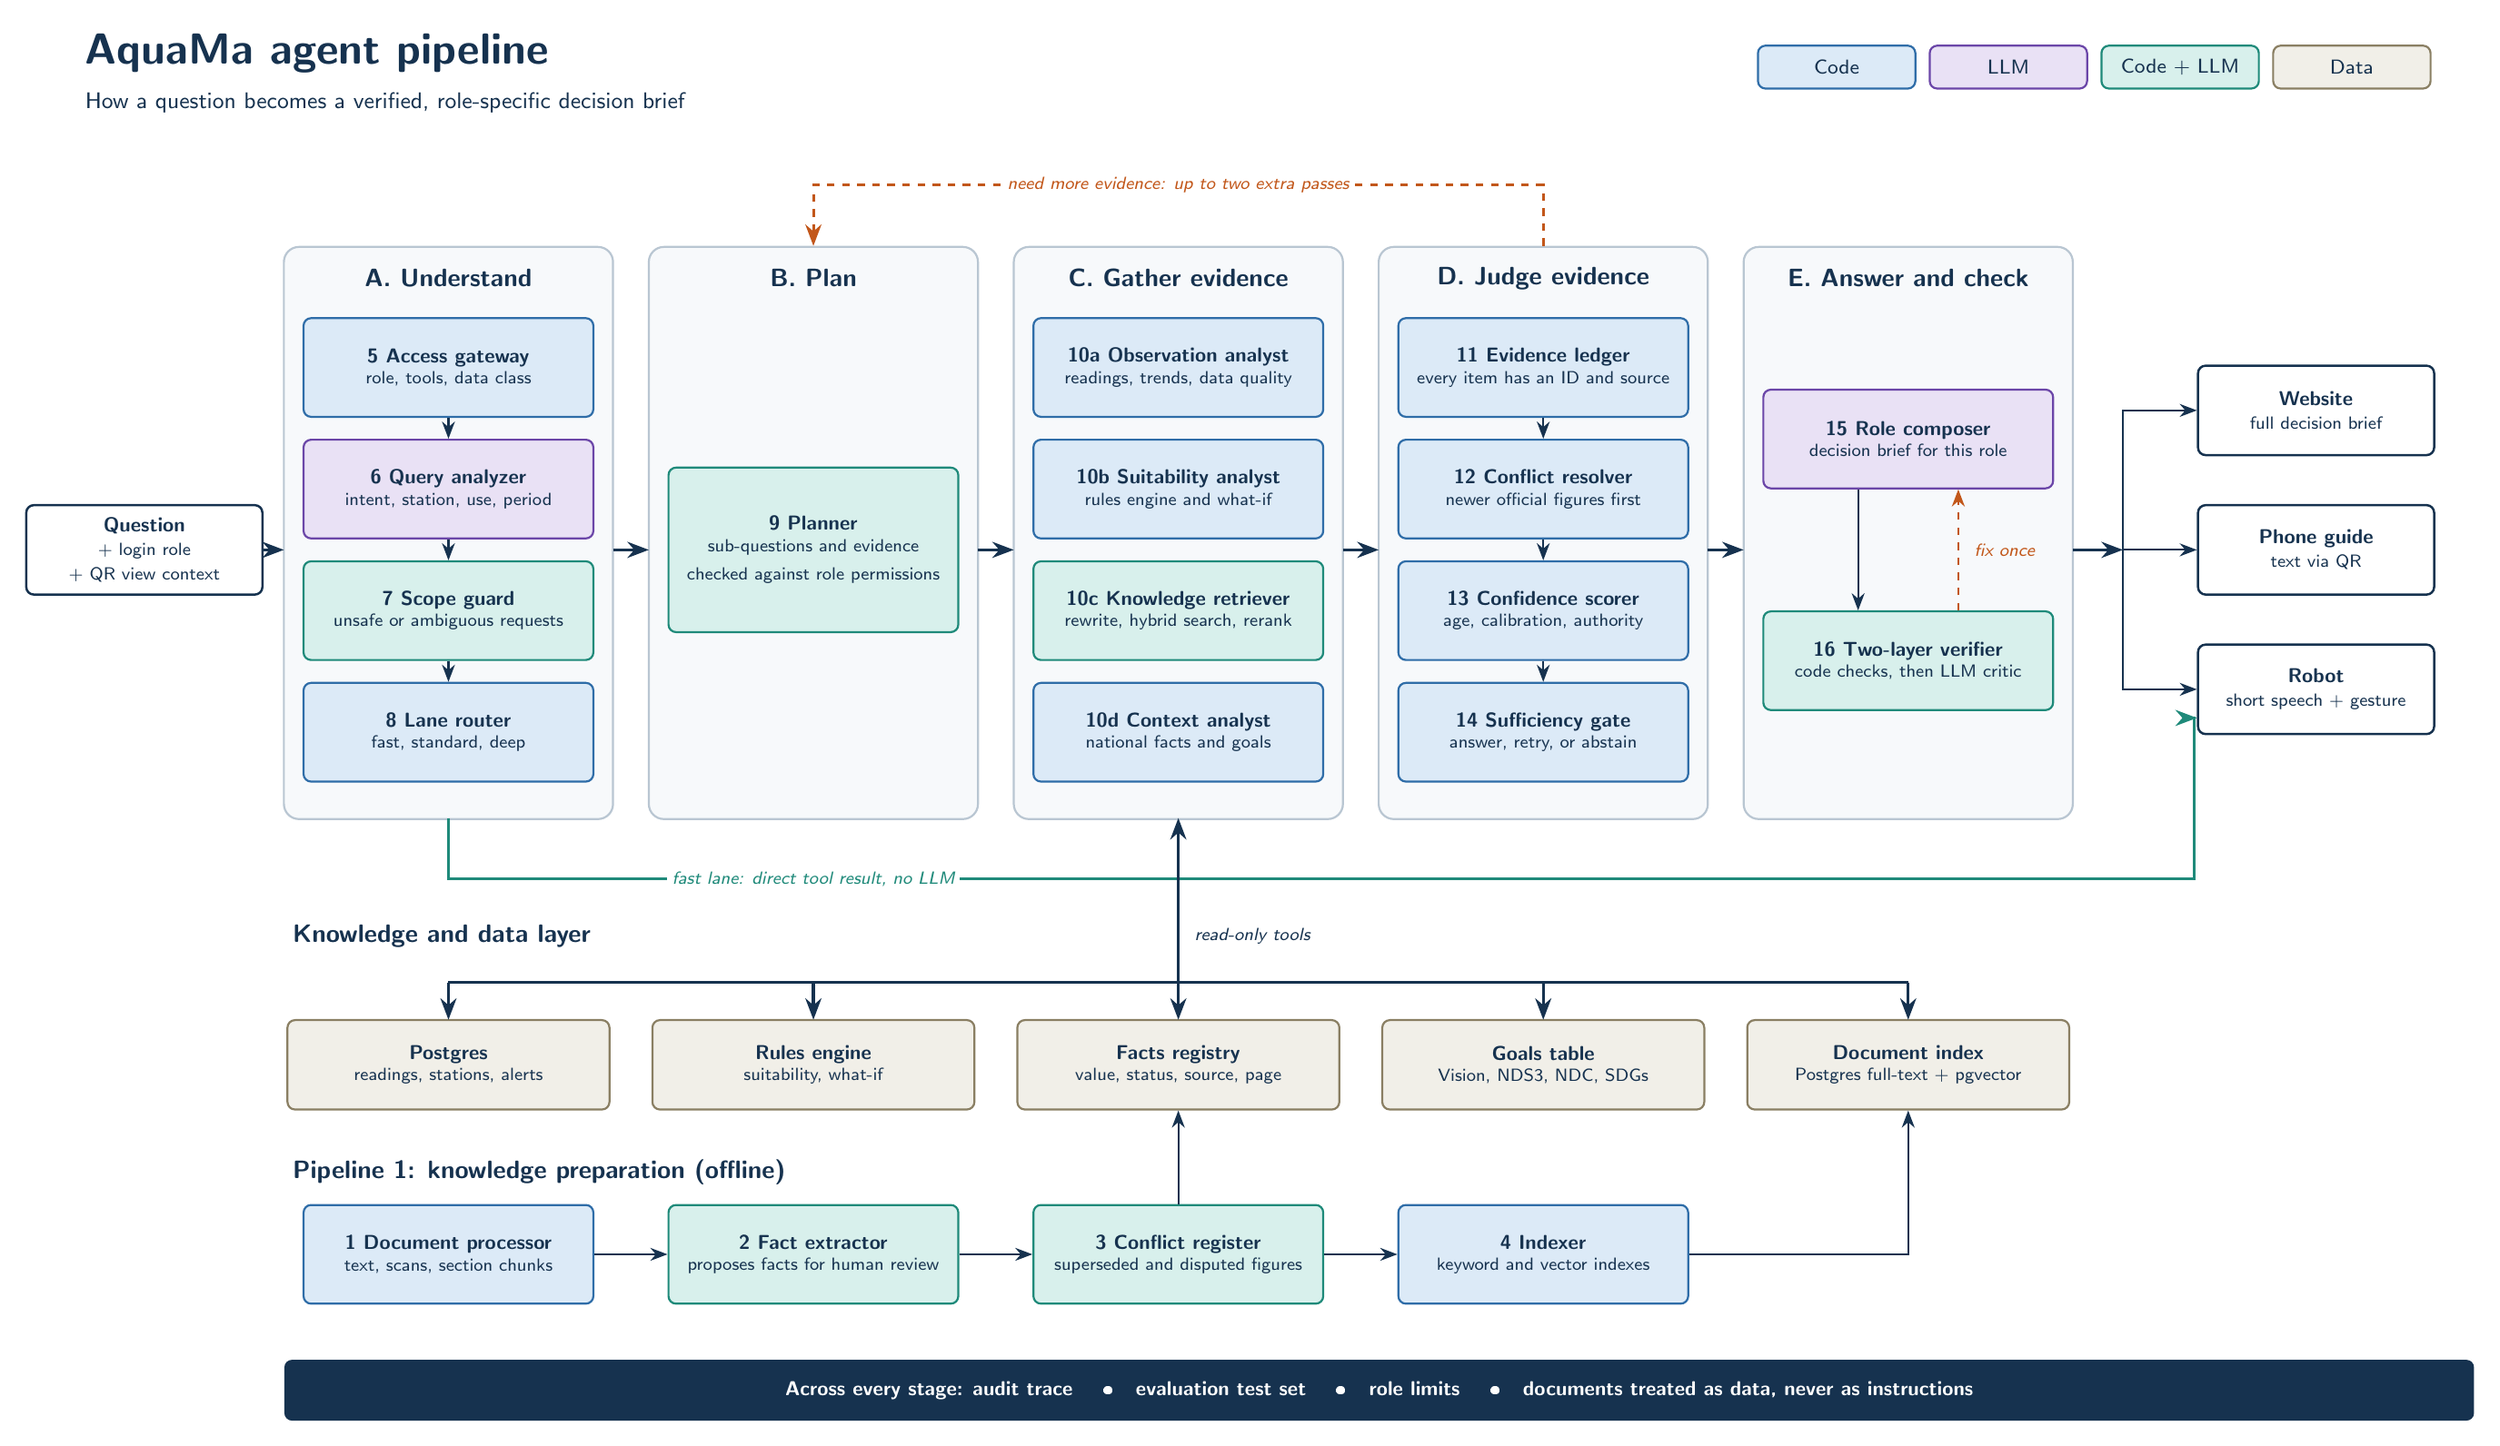
\begin{tikzpicture}

% title
\node[anchor=west,font=\LARGE\bfseries,text=ink] at (0,20.3) {AquaMa agent pipeline};
\node[anchor=west,font=\small,text=ink] at (0,19.6) {How a question becomes a verified, role-specific decision brief};

% legend
\node[code,minimum width=2.2cm,minimum height=0.6cm] at (24.6,20.1) {Code};
\node[llm,minimum width=2.2cm,minimum height=0.6cm] at (27.0,20.1) {LLM};
\node[mix,minimum width=2.2cm,minimum height=0.6cm] at (29.4,20.1) {Code + LLM};
\node[store,minimum width=2.2cm,minimum height=0.6cm] at (31.8,20.1) {Data};

% stages
\foreach \x/\t in {5.2/A. Understand,10.3/B. Plan,15.4/C. Gather evidence,20.5/D. Judge evidence,25.6/E. Answer and check}{
  \node[stagebox,minimum width=4.6cm,minimum height=8.0cm,anchor=north] at (\x,17.6) {};
  \node[stagetitle] at (\x,17.15) {\t};
}

% stage A
\node[code] (gate) at (5.2,15.9) {\cname{5 Access gateway}{role, tools, data class}};
\node[llm]  (qa)   at (5.2,14.2) {\cname{6 Query analyzer}{intent, station, use, period}};
\node[mix]  (scope)at (5.2,12.5) {\cname{7 Scope guard}{unsafe or ambiguous requests}};
\node[code] (lane) at (5.2,10.8) {\cname{8 Lane router}{fast, standard, deep}};
\draw[soft] (gate)--(qa); \draw[soft] (qa)--(scope); \draw[soft] (scope)--(lane);

% stage B
\node[mix,minimum height=2.3cm] (plan) at (10.3,13.35) {\cname{9 Planner}{sub-questions and evidence}\\[2pt]{\scriptsize checked against role permissions}};

% stage C
\node[code] (obs) at (15.4,15.9) {\cname{10a Observation analyst}{readings, trends, data quality}};
\node[code] (suit)at (15.4,14.2) {\cname{10b Suitability analyst}{rules engine and what-if}};
\node[mix]  (ret) at (15.4,12.5) {\cname{10c Knowledge retriever}{rewrite, hybrid search, rerank}};
\node[code] (ctx) at (15.4,10.8) {\cname{10d Context analyst}{national facts and goals}};

% stage D
\node[code] (led) at (20.5,15.9) {\cname{11 Evidence ledger}{every item has an ID and source}};
\node[code] (con) at (20.5,14.2) {\cname{12 Conflict resolver}{newer official figures first}};
\node[code] (sco) at (20.5,12.5) {\cname{13 Confidence scorer}{age, calibration, authority}};
\node[code] (suf) at (20.5,10.8) {\cname{14 Sufficiency gate}{answer, retry, or abstain}};
\draw[soft] (led)--(con); \draw[soft] (con)--(sco); \draw[soft] (sco)--(suf);

% stage E
\node[llm] (comp) at (25.6,14.9) {\cname{15 Role composer}{decision brief for this role}};
\node[mix] (ver)  at (25.6,11.8) {\cname{16 Two-layer verifier}{code checks, then LLM critic}};
\draw[soft] ([xshift=-7mm]comp.south)--([xshift=-7mm]ver.north);
\draw[-{Stealth[length=2.4mm]},line width=0.9pt,draw=warn,dashed] ([xshift=7mm]ver.north)--([xshift=7mm]comp.south);
\node[note,text=warn,anchor=west] at (26.4,13.35) {fix once};

% input and output
\node[io] (in) at (0.95,13.35) {\textbf{Question}\\{\scriptsize + login role}\\{\scriptsize + QR view context}};
\node[io] (web) at (31.3,15.3) {\textbf{Website}\\{\scriptsize full decision brief}};
\node[io] (ph)  at (31.3,13.35) {\textbf{Phone guide}\\{\scriptsize text via QR}};
\node[io] (rob) at (31.3,11.4) {\textbf{Robot}\\{\scriptsize short speech + gesture}};

% main flow
\draw[flow] (in.east)--(2.9,13.35);
\draw[flow] (7.5,13.35)--(8.0,13.35);
\draw[flow] (12.6,13.35)--(13.1,13.35);
\draw[flow] (17.7,13.35)--(18.2,13.35);
\draw[flow] (22.8,13.35)--(23.3,13.35);
\draw[flow] (27.9,13.35)--(28.6,13.35);
\draw[soft] (28.6,13.35)--(ph.west);
\draw[soft] (28.6,13.35)|-(web.west);
\draw[soft] (28.6,13.35)|-(rob.west);

% retry loop
\draw[loop] (20.5,17.6)--(20.5,18.45)--(10.3,18.45)--(10.3,17.6);
\node[note,text=warn,fill=white,inner sep=2pt] at (15.4,18.45) {need more evidence: up to two extra passes};

% fast lane
\draw[-{Stealth[length=3mm]},line width=1.1pt,draw=mixB] (5.2,9.6)--(5.2,8.75)--(29.6,8.75)--(29.6,11.0)--(rob.west |- 0,11.0);
\node[note,text=mixB,fill=white,inner sep=2pt] at (10.3,8.75) {fast lane: direct tool result, no LLM};

% knowledge layer
\node[anchor=west,stagetitle] at (2.9,7.95) {Knowledge and data layer};
\node[store] (d1) at (5.2,6.15)  {\cname{Postgres}{readings, stations, alerts}};
\node[store] (d2) at (10.3,6.15) {\cname{Rules engine}{suitability, what-if}};
\node[store] (d3) at (15.4,6.15) {\cname{Facts registry}{value, status, source, page}};
\node[store] (d4) at (20.5,6.15) {\cname{Goals table}{Vision, NDS3, NDC, SDGs}};
\node[store] (d5) at (25.6,6.15) {\cname{Document index}{Postgres full-text + pgvector}};
\draw[line width=1.2pt,draw=ink] (5.2,7.3)--(25.6,7.3);
\foreach \x in {5.2,10.3,15.4,20.5,25.6}{\draw[flow] (\x,7.3)--(\x,6.78);}
\draw[flow,{Stealth[length=3mm]}-] (15.4,9.6)--(15.4,7.3);
\node[note,fill=white,inner sep=2pt,anchor=west] at (15.55,7.95) {read-only tools};

% pipeline 1
\node[anchor=west,stagetitle] at (2.9,4.65) {Pipeline 1: knowledge preparation (offline)};
\node[code] (p1) at (5.2,3.5)  {\cname{1 Document processor}{text, scans, section chunks}};
\node[mix]  (p2) at (10.3,3.5) {\cname{2 Fact extractor}{proposes facts for human review}};
\node[mix]  (p3) at (15.4,3.5) {\cname{3 Conflict register}{superseded and disputed figures}};
\node[code] (p4) at (20.5,3.5) {\cname{4 Indexer}{keyword and vector indexes}};
\draw[soft] (p1)--(p2); \draw[soft] (p2)--(p3); \draw[soft] (p3)--(p4);
\draw[soft] (p3.north)--(d3.south);
\draw[soft] (p4.east)-|(d5.south);

% cross cutting
\node[rounded corners=3pt,fill=ink,text=white,minimum width=30.6cm,minimum height=0.85cm,font=\footnotesize\bfseries,anchor=west] at (2.9,1.6)
  {Across every stage: audit trace \quad\textbullet\quad evaluation test set \quad\textbullet\quad role limits \quad\textbullet\quad documents treated as data, never as instructions};

\end{tikzpicture}
\end{document}
